\documentclass[12pt,]{article}
\usepackage[utf8]{inputenc}
\usepackage[T1]{fontenc}
\usepackage{mathptmx}
\usepackage{geometry}
\usepackage{mathtools}
\usepackage[english]{babel}
\usepackage{graphicx}
\usepackage{stackengine}
\usepackage[os=win]{menukeys}
\usepackage{hyperref}
\usepackage{minted}
\usepackage{xcolor}
\usepackage{tikz}
\usepackage[yyyymmdd,hhmmss]{datetime}
\usepackage{etoolbox}

\patchcmd{\thebibliography}{\section*{\refname}}{}{}{}

\newcommand{\ShowOsVersion}{
	\immediate\write18{\unexpanded{foo=`uname -sro` && echo "${foo}" > tmp.tex}}
	\input{tmp}\immediate\write18{rm tmp.tex}
}

\newcommand{\ShowTexVersion}{
	\immediate\write18{\unexpanded{foo=`pdflatex -version | head -n1 | cut -d' ' -f1,2` && echo "${foo}" > tmp.tex}}
	\input{tmp}\immediate\write18{rm tmp.tex}
}

\addto\captionsenglish{\renewcommand{\contentsname}{Daftar Isi}}

\hypersetup{
	colorlinks=true, %set true if you want colored links
	linktoc=all,     %set to all if you want both sections and subsections linked
	linkcolor=blue,  %choose some color if you want links to stand out
}

\geometry{
	legalpaper,
	left=15mm,
	right=10mm,
	top=10mm,
	bottom=15mm,
}

\title{\Large \bf
	License and Patent Claim Draft\\
	\small{(Mid-Testing Stage)}
}

\author{Achmadi ST MT}

\date{}

\hypersetup{citecolor=black}

\definecolor{LightGray}{gray}{0.95}

%\pagecolor[rgb]{0.1,0.1,0.1}
%\color[rgb]{1,1,1}

\begin{document}
	\maketitle
	\thispagestyle{empty}
	
	\vspace*{600pt}
	\noindent Seluruh konten dalam dokumen ini mengacu kepada pengembangan unit Audiometri di \textit{commit} terakhir:\\
	\url{https://github.com/VibrasticLab/pikoakustik/commit/fa1db9a040644eab3fd033c1f8c43e28af1f0ebf}.\\
	
	\noindent This report written using: \\
	OS : \ShowOsVersion \\
	TeX : \ShowTexVersion \\
	Update: {\today} at \currenttime \\
	
	%%%%%%%%%%%%%%%%%%%%%%%%%%%%%%%%%%%%%%%%%%%%%%%%%%%%%%%%%%%%%%%%%
	
	\newpage
	\tableofcontents
	
	%%%%%%%%%%%%%%%%%%%%%%%%%%%%%%%%%%%%%%%%%%%%%%%%%%%%%%%%%%%%%%%%%
	
	\newpage
	\section{Software/Firmware}
	
	Berikut akan dijabarkan beberapa aspek dari sisi software/firmware yang dijalankan di hardware.
	Seluruh klaim pada aspek ini dalam bentuk klaim kode sumber (\textit{source-code}) dan tidak terbatas hanya \textit{binary} akhir.
	
	\subsection{Libraries}
	Disini akan dijabarkan pengunaan pustaka (libraries) yang digunakan dalam pengembangan.
	Seluruh pustaka disini berupa kode sumber implementasi dan API (\textit{Application Programming Interface})
	di luar implementasi dan perbaikan (\textit{patch}) yang dilakukan oleh pihak peneliti disini.
	
	Penjabaran ini perlu mengingat pustaka tersebut dikembangankan oleh pihak lain dan telah memiliki klaim lisensi sendiri.
	Sehingga secara otomatis pihak peneliti disini \textbf{tidak bisa mengklaim} pustaka tersebut.
	
	\begin{itemize}
		\item \textbf{GNU GCC ARM}. Merupakan sekumpulan \textit{toolchain} dan pustaka untuk kompilasi source-code ke binary untuk chip ARM.
		Dikembangan oleh ARM Limited dengan lisensi yang digunakan adalah GPL versi 3.0\\
		\url{https://developer.arm.com/open-source/gnu-toolchain/gnu-rm}
		
		\item \textbf{ChibiOS/RT}. Merupakan sekumpulan pustaka yang berisi implementasi dan API abstraksi untuk chip ARM seri Cortex-M.
		Dikembangkan oleh Giovanni Di Sirio dengan lisensi yang digunakan adalah GPL versi 3.0 dan Apache versi 2.0\\
		\url{https://www.chibios.org/dokuwiki/doku.php}
		
		\item \textbf{FatFS}. Merupakan sekumpulan pustaka yang berisi implementasi dan API abstraksi untuk FAT16/FAT32 \textit{filesystem}.
		Pustaka ini digunakan untuk menangani berkas-berkas teks yang disimpan di \textit{memory-card}.
		Dikembangkan oleh Elm ChanN dengan lisensi yang digunakan adalah BSD license.\\
		\url{http://elm-chan.org/fsw/ff/00index_e.html}
		
		\item \textbf{ESP-Open-SDK}. Merupakan sekumpulan \textit{toolchain} dan pustaka untuk kompilasi source-code ke binary untuk platform ESP8266/EX.
		Dikembangan oleh Tensilica Inc. dan Espressif Inc. dengan lisensi yang digunakan adalah GPL versi 2.0\\
		\url{https://github.com/pfalcon/esp-open-sdk}
		
		\item \textbf{esp\_mqtt}. Merupakan sekumpulan pustaka yang berisi implementasi protocol MQTT Client untuk ESP8266/EX.
		Dikembangkan oleh Tuan PM dengan lisensi yang digunakan adalah MIT License.\\
		\url{https://github.com/tuanpmt/esp_mqtt}
	\end{itemize}

	\subsection{Audio}
	
	Berikut dijabarkan beberapa klaim terhadap referensi metode/algoritma terkait fitur Audio/Tone.
	eluruh referensi dapat ditemukan pada berkas sumber \textbf{ht\_audio.c}.
	
	\subsubsection{Tone Generation}
	
	Referensi persamaan untuk \textit{tone generation}.
	Aspek klaim adalah pola persamaan dan seluruh definisi konstanta yang digunakan,
	terkecuali objek struktur konfigurasi I2S.
	
	\begin{minted}[frame=lines,framesep=2mm,fontsize=\small,bgcolor=LightGray]{c}
#define USE_STEREO_ARRAY TRUE

#define I2S_BUFF_SIZE 512
#define DEFAULT_ATTEN 0.01
#define DEFAULT_AMPL_THD 1

#define TOTAL_BUFF_SIZE I2S_BUFF_SIZE*16

void ht_audio_Zero(void){
	uint16_t i;
	for(i=0;i<TOTAL_BUFF_SIZE;i++){
		i2s_tx_buf[i] = 0;
	}
}

void ht_audio_Tone(double freq, double ampl){
	uint16_t i;
	uint16_t buffsize;
	double ysin;
	double ampl_act;
	
	buffsize = (uint16_t) I2S_BUFF_SIZE/freq;
	
	ampl_act = DEFAULT_ATTEN*ampl*32767;
	if(ampl_act<=DEFAULT_AMPL_THD){ampl = 0;}
	
	ht_audio_Zero();
	
	for(i=0;i<buffsize;i++){
		ysin = DEFAULT_ATTEN*ampl*32767*sin(2*3.141592653589793*((double)i/(double)buffsize));
	
		if(ysin >= 0){
			i2s_tx_buf[i]=ysin;
#if USE_STEREO_ARRAY
			i2s_tx_buf[i+1]=ysin;
#endif
	}
		if(ysin < 0){
			i2s_tx_buf[i]=ysin+65535;
#if USE_STEREO_ARRAY
			i2s_tx_buf[i+1]=ysin+65535;
#endif
		}
	}
	
	i2scfg.size = buffsize; //Can't claimed
}
	\end{minted}

	\subsubsection{Tone Play}
	
	Referensi metode untuk \textit{tone playing}.
	Aspek klaim adalah durasi dan flow metode, terkecuali objek struktur konfigurasi I2S.

\begin{minted}[frame=lines,framesep=2mm,fontsize=\small,bgcolor=LightGray]{c}
void ht_audio_Play(uint16_t duration){
	i2sStart(&I2SD2, &i2scfg);
	i2sStartExchange(&I2SD2);
	
	chThdSleepMilliseconds(duration*10);
	
	i2sStopExchange(&I2SD2);
	i2sStop(&I2SD2);
}
\end{minted}

	\subsubsection{L/R Control}
	
	Referensi metode untuk kendali channel kiri-kanan.
	Aspek klaim adalah flow metode, terkecuali nomor pin pada chip STM32.
	
	\begin{minted}[frame=lines,framesep=2mm,fontsize=\small,bgcolor=LightGray]{c}
void ht_audio_Init(void){
	palSetPadMode(AUDIO_IO,AUDIO_L,PAL_MODE_OUTPUT_PUSHPULL);
	palSetPadMode(AUDIO_IO,AUDIO_R,PAL_MODE_OUTPUT_PUSHPULL);
}
	
void ht_audio_DisableCh(void){
	palClearPad(AUDIO_IO,AUDIO_L);
	palClearPad(AUDIO_IO,AUDIO_R);
}

void ht_audio_LeftCh(void){
	ht_audio_DisableCh();
	palSetPad(AUDIO_IO,AUDIO_L);
}

void ht_audio_RightCh(void){
	ht_audio_DisableCh();
	palSetPad(AUDIO_IO,AUDIO_R);
}
	\end{minted}
	
	\newpage
	\subsection{Serial Commands}
	
	Berikut dijabarkan beberapa klaim terhadap referensi metode/algoritma terkait fitur Serial Commands yang dapat diakses melalu jalur USB-CDC.
	Seluruh referensi dapat ditemukan pada berkas sumber \textbf{ht\_comm.c}
	
	\subsubsection{Testing}
	Perintah untuk menjalankan rutin testing baik untuk komunikasi serial dan audio
	\begin{minted}[frame=lines,framesep=2mm,fontsize=\small,bgcolor=LightGray]{bash}
ch> test [0|1]
	\end{minted}

	\begin{minted}[frame=lines,framesep=2mm,fontsize=\small,bgcolor=LightGray]{c}
static void cmd_test(BaseSequentialStream *chp, int argc, char *argv[]) {
	uint8_t lrc;
	
	chprintf(chp,"Serial Console at %d & buffer size %d bit\r\n",SERIAL_DEFAULT_BITRATE,SERIAL_BUFFERS_SIZE);
	chprintf(chp,"Playing Audio Test\r\n");
	
	if(argc==0){
#if USER_AUDIO
		chprintf(chp,"Test on both Channel\r\n");
		ht_audio_TestBoth();
#else
	chprintf(chp,"Audio features disabled\r\n");
#endif
	}
	else if(argc == 1){
#if USER_AUDIO
		lrc = atoi(argv[0]);
		ht_audio_Tone(1.25,1);
	
		if(lrc==OUT_LEFT){
			ht_audio_LeftCh();
			chprintf(chp,"Test on Left Channel\r\n");
			ht_audio_Play(TEST_DURATION);
			chThdSleepMilliseconds(200);
			ht_audio_Play(TEST_DURATION);
		}
		else if(lrc==OUT_RIGHT){
			ht_audio_RightCh();
			chprintf(chp,"Test on Right Channel\r\n");
			ht_audio_Play(TEST_DURATION);
			chThdSleepMilliseconds(200);
			ht_audio_Play(TEST_DURATION);
		}
		else{
			chprintf(chp,"Channel option incorrect \r\n");
		}
		ht_audio_DisableCh();
#else
		chprintf(chp,"Audio features disabled\r\n");
#endif
	}
	else{
		chprintf(chp,"usage: test [0|1] \r\n");
		chprintf(chp,"0 -> Left Channel \r\n");
		chprintf(chp,"1 -> Righ Channel \r\n");
		return;
	}
}
	\end{minted}

	\newpage
	\subsubsection{Audio: Zero}
	Perintah untuk menjalankan rutin testing tone pada 0 dBV.
	\begin{minted}[frame=lines,framesep=2mm,fontsize=\small,bgcolor=LightGray]{bash}
ch> zero [0/1]
	\end{minted}

	\begin{minted}[frame=lines,framesep=2mm,fontsize=\small,bgcolor=LightGray]{c}
static void cmd_zero(BaseSequentialStream *chp, int argc, char *argv[]) {
	if(argc != 1){chprintf(chp,"usage: zero <0/1>\r\n");return;}
	
	uint8_t lrc = atoi(argv[0]);
	switch(lrc){
	case OUT_LEFT:
		ht_audio_LeftCh();
		chprintf(chp,"Left Channel on\r\n");
		break;
	
	case OUT_RIGHT:
		ht_audio_RightCh();
		chprintf(chp,"Right Channel on\r\n");
		break;
	}
	
	chprintf(chp,"Test Audio: Sine Zero\r\n");
	ht_audio_Tone(1.25,0);
	ht_audio_Play(TEST_DURATION);
	ht_audio_DisableCh();
	chprintf(chp,"Finished\r\n");
}
	\end{minted}

	\subsubsection{Audio: Max}
	Perintah untuk menjalankan rutin testing tone pada dBV maximum.
	\begin{minted}[frame=lines,framesep=2mm,fontsize=\small,bgcolor=LightGray]{bash}
ch> max [0/1]
	\end{minted}

	\begin{minted}[frame=lines,framesep=2mm,fontsize=\small,bgcolor=LightGray]{c}
static void cmd_max(BaseSequentialStream *chp, int argc, char *argv[]) {
	if(argc != 1){chprintf(chp,"usage: max <0/1>\r\n");return;}
	
	uint8_t lrc = atoi(argv[0]);
	switch(lrc){
		case OUT_LEFT:
			ht_audio_LeftCh();
			chprintf(chp,"Left Channel on\r\n");
			break;
		
		case OUT_RIGHT:
			ht_audio_RightCh();
			chprintf(chp,"Right Channel on\r\n");
			break;
	}
	
	chprintf(chp,"Test Audio: Sine Maximum\r\n");
	ht_audio_Tone(1.25,1);
	ht_audio_Play(TEST_DURATION);
	ht_audio_DisableCh();
	chprintf(chp,"Finished\r\n");
}
	\end{minted}
	
	\subsubsection{Audio: Min}
	Perintah untuk menjalankan rutin testing tone pada dBV minimum.
	\begin{minted}[frame=lines,framesep=2mm,fontsize=\small,bgcolor=LightGray]{bash}
ch> min [0/1]
	\end{minted}

	\begin{minted}[frame=lines,framesep=2mm,fontsize=\small,bgcolor=LightGray]{c}
static void cmd_min(BaseSequentialStream *chp, int argc, char *argv[]) {
	if(argc != 1){chprintf(chp,"usage: min <0/1>\r\n");return;}
	
	uint8_t lrc = atoi(argv[0]);
	switch(lrc){
		case OUT_LEFT:
			ht_audio_LeftCh();
			chprintf(chp,"Left Channel on\r\n");
			break;
		
		case OUT_RIGHT:
			ht_audio_RightCh();
			chprintf(chp,"Right Channel on\r\n");
			break;
	}
	
	chprintf(chp,"Test Audio: Sine Minimum\r\n");
	ht_audio_Tone(1.25,SMALLEST_DB);
	ht_audio_Play(TEST_DURATION);
	ht_audio_DisableCh();
	chprintf(chp,"Finished\r\n");
}
	\end{minted}

	\subsubsection{Audio: Tone}
	Perintah untuk menjalankan rutin testing tone pada skala frekuensi dan amplitud tertentu.
	\begin{minted}[frame=lines,framesep=2mm,fontsize=\small,bgcolor=LightGray]{bash}
ch> tone <0/1> <freq> <ampl>
	\end{minted}

	\begin{minted}[frame=lines,framesep=2mm,fontsize=\small,bgcolor=LightGray]{c}
static void cmd_tone(BaseSequentialStream *chp, int argc, char *argv[]) {
	double vampl;
	double vfreq;
	uint8_t lrc = 0;
	uint16_t sing_durr = 500;
	
	if(argc==2){
		lrc = 0;
		vfreq = atof(argv[0]);
		vampl = atof(argv[1]);
	}
	else if(argc==3){
		lrc = atoi(argv[0]);
		vfreq = atof(argv[1]);
		vampl = atof(argv[2]);
	}
	else{
		chprintf(chp,"usage: tone <0/1> <freq> <ampl>\r\n");
		return;
	}
	
	switch(lrc){
		case OUT_LEFT:
			ht_audio_LeftCh();
			chprintf(chp,"Left Channel on\r\n");
			break;
		
		case OUT_RIGHT:
			ht_audio_RightCh();
			chprintf(chp,"Right Channel on\r\n");
			break;
	}
	
	if(vampl<=SMALLEST_DB){
		chprintf(chp,"Warning: Amplitude bellow smallest set\r\n");
	}
	
	chprintf(chp,"Tone: Freq:%6.4f Ampl:%6.4f\r\n",vfreq,vampl);
	ht_audio_Tone(vfreq,vampl);
	ht_audio_Play(sing_durr);
	chprintf(chp,"Finished\r\n");
	ht_audio_DisableCh();
}
	\end{minted}
	
	\subsubsection{Audio: Sing}
	Perintah untuk menjalankan rutin testing tone skala tertinggi hingga terendah pada skala frekuensi tertentu.
	\begin{minted}[frame=lines,framesep=2mm,fontsize=\small,bgcolor=LightGray]{bash}
ch> sing <0/1> <freq>
	\end{minted}
	
	\begin{minted}[frame=lines,framesep=2mm,fontsize=\small,bgcolor=LightGray]{c}
static void cmd_sing(BaseSequentialStream *chp, int argc, char *argv[]) {
	double vampl = 1;
	double vfreq = 1.25;
	uint8_t lrc = 0;
	uint16_t sing_durr = 500;
	
	if(argc == 0){
		lrc = 0;
		vfreq = 1.25;
	}
	else if(argc == 1){
		lrc = 0;
		vfreq = atof(argv[0]);
	}
	else if(argc == 2){
		lrc = atoi(argv[0]);
		vfreq = atof(argv[1]);
	}
	else{
		chprintf(chp,"usage: sing <0/1> <freq>\r\n");return;
	}
	
	switch(lrc){
		case OUT_LEFT:
			ht_audio_LeftCh();
			chprintf(chp,"Left Channel on\r\n");
			break;
			
		case OUT_RIGHT:
			ht_audio_RightCh();
			chprintf(chp,"Right Channel on\r\n");
			break;
	}
	
	while(1){
		chprintf(chp,"Sing: Freq:%6.4f Ampl:%6.4f\r\n",vfreq,vampl);
		ht_audio_Tone(vfreq,vampl);
		ht_audio_Play(sing_durr);
		chThdSleepMilliseconds(500);
		
		vampl = vampl/2;
		if(vampl<SMALLEST_DB){
			chprintf(chp,"Finished\r\n");
			break;
		}
	}
	ht_audio_DisableCh();
}
	\end{minted}
	
	\newpage
	\subsubsection{Audio: Speaker Test}
	Perintah untuk menjalankan rutin testing speaker dengan dua tone berurutan.
	Referensi tone di berkas \textbf{ht\_audio.c}.
	\begin{minted}[frame=lines,framesep=2mm,fontsize=\small,bgcolor=LightGray]{bash}
ch> sptest <0/1/2>
	\end{minted}
	
	\begin{minted}[frame=lines,framesep=2mm,fontsize=\small,bgcolor=LightGray]{c}
static void cmd_sptest(BaseSequentialStream *chp, int argc, char *argv[]) {
	uint8_t lrc;
	
	if(argc != 1){chprintf(chp,"usage: sptest <0/1/2>\r\n");return;}
	
	lrc = atoi(argv[0]);
	
	switch(lrc){
		case 0: chprintf(chp,"Testing Left Channel\r\n"); ht_audio_TestLeft();break;
		case 1: chprintf(chp,"Testing Right Channel\r\n"); ht_audio_TestRight();break;
		case 2: chprintf(chp,"Testing Both Channel\r\n"); ht_audio_TestBoth();break;
	}
}
	\end{minted}
	
	\subsubsection{MMC: List Files}
	Perintah untuk menjalankan menampilkan daftar file yang tersimpan di MMC.
	Referensi metode MMC di berkas \textbf{ht\_mmc.c}.
	\begin{minted}[frame=lines,framesep=2mm,fontsize=\small,bgcolor=LightGray]{bash}
ch> ls
	\end{minted}
	
	\begin{minted}[frame=lines,framesep=2mm,fontsize=\small,bgcolor=LightGray]{c}
static void cmd_lsfile(BaseSequentialStream *chp, int argc, char *argv[]) {
	(void) argv;
	if(argc != 0){chprintf(chp,"usage: ls\r\n");return;}
	
	ht_mmc_lsFiles();
}
	}
	\end{minted}
	
	\subsubsection{MMC: Show File}
	Perintah untuk menjalankan menampilkan isi file yang tersimpan di MMC pada nomer tertentu.
	Referensi metode MMC di berkas \textbf{ht\_mmc.c}.
	\begin{minted}[frame=lines,framesep=2mm,fontsize=\small,bgcolor=LightGray]{bash}
ch> cat [N]
	\end{minted}
	
	\begin{minted}[frame=lines,framesep=2mm,fontsize=\small,bgcolor=LightGray]{c}
static void cmd_catfile(BaseSequentialStream *chp, int argc, char *argv[]) {
	(void) argv;
	uint8_t fnum;
	
	if(argc==0 || argc>1){chprintf(chp,"usage: cat file_number\r\n");return;}
		fnum = atoi(argv[0]);
		ht_mmc_catFiles(fnum);
}
	\end{minted}
	
	\subsubsection{MMC: Test Write}
	Perintah untuk menjalankan rutin test Read/Write di MMC.
	Referensi metode MMC di berkas \textbf{ht\_mmc.c}.
	\begin{minted}[frame=lines,framesep=2mm,fontsize=\small,bgcolor=LightGray]{bash}
ch> mmc
	\end{minted}
	
	\begin{minted}[frame=lines,framesep=2mm,fontsize=\small,bgcolor=LightGray]{c}
static void cmd_mmcwrt(BaseSequentialStream *chp, int argc, char *argv[]) {
	(void) argv;
	if(argc != 0){chprintf(chp,"usage: mmcwr\r\n");return;}
	
	ht_mmc_Test();
	chprintf(chp,"MMC R/W Test Finished\r\n\r\n");
}
	\end{minted}
	
	\subsubsection{MMC: Show Contents}
	Perintah untuk menjalankan rutin test File Read di MMC.
	Referensi metode MMC di berkas \textbf{ht\_mmc.c}.
	\begin{minted}[frame=lines,framesep=2mm,fontsize=\small,bgcolor=LightGray]{bash}
ch> mmcat
	\end{minted}
	
	\begin{minted}[frame=lines,framesep=2mm,fontsize=\small,bgcolor=LightGray]{c}
static void cmd_mmcat(BaseSequentialStream *chp, int argc, char *argv[]) {
	(void) argv;
	if(argc != 0){chprintf(chp,"usage: mmcat\r\n");return;}
	
	ht_mmc_catTest();
	chprintf(chp,"MMC R/W Content look Finished\r\n\r\n");
}
	\end{minted}
	
	\subsubsection{MMC: Check MMC}
	Perintah untuk menjalankan rutin test \textit{filesystem} di MMC.
	Referensi metode MMC di berkas \textbf{ht\_mmc.c}.
	\begin{minted}[frame=lines,framesep=2mm,fontsize=\small,bgcolor=LightGray]{bash}
ch> mmcat
	\end{minted}
	
	\begin{minted}[frame=lines,framesep=2mm,fontsize=\small,bgcolor=LightGray]{c}
static void cmd_mmchk(BaseSequentialStream *chp, int argc, char *argv[]) {
	(void) argv;
	if(argc != 0){chprintf(chp,"usage: mmchk\r\n");return;}
	
	ht_mmc_initCheck();
	chprintf(chp,"MMC Checking Finished\r\n\r\n");
}
	\end{minted}
	
	\subsubsection{IOT: MQTT Subscribe}
	Perintah untuk menjalankan rutin test subscribe via MQTT.
	Referensi metode MMC di \textit{source-tree} proyek \textbf{esp8266dev}.
	\begin{minted}[frame=lines,framesep=2mm,fontsize=\small,bgcolor=LightGray]{bash}
ch> sub
	\end{minted}
	
	\begin{minted}[frame=lines,framesep=2mm,fontsize=\small,bgcolor=LightGray]{c}
static void cmd_iotsub(BaseSequentialStream *chp, int argc, char *argv[]) {
	(void) argv;
	if(argc != 0){chprintf(chp,"usage: sub\r\n");return;}
	
	ht_comm_IoT("sub\r\n");
	chprintf(chp,"IoT subscribe hello/world Finished\r\n\r\n");
}
	\end{minted}
	
	\subsubsection{IOT: MQTT Publish}
	Perintah untuk menjalankan rutin test Publish via MQTT.
	Referensi metode MMC di \textit{source-tree} proyek \textbf{esp8266dev}.
	\begin{minted}[frame=lines,framesep=2mm,fontsize=\small,bgcolor=LightGray]{bash}
ch> pub
	\end{minted}
	
	\begin{minted}[frame=lines,framesep=2mm,fontsize=\small,bgcolor=LightGray]{c}
static void cmd_iotpub(BaseSequentialStream *chp, int argc, char *argv[]) {
	(void) argv;
	if(argc != 0){chprintf(chp,"usage: pub\r\n");return;}
	
	ht_comm_IoT("pub\r\n");
	chprintf(chp,"IoT publish hello/world Finished\r\n\r\n");
}
	\end{minted}
	
	\subsubsection{IOT: MQTT Send HTTP JSON}
	Perintah untuk menjalankan rutin test kirim JSON hasil ke server via HTTPS.
	Referensi metode MMC di \textit{source-tree} proyek \textbf{esp8266dev}.
	\begin{minted}[frame=lines,framesep=2mm,fontsize=\small,bgcolor=LightGray]{bash}
ch> send
	\end{minted}
	
	\begin{minted}[frame=lines,framesep=2mm,fontsize=\small,bgcolor=LightGray]{c}
static void cmd_iotsend(BaseSequentialStream *chp, int argc, char *argv[]) {
	(void) argv;
	if(argc != 0){chprintf(chp,"usage: send\r\n");return;}
	
	ht_mmc_lsFiles();
	ht_mmc_sendFiles(lastnum);
	ht_comm_IoT("send\r\n");
}
	\end{minted}
	
	\subsubsection{IOT: MQTT Send MQTT Result Log}
	Perintah untuk menjalankan rutin test kirim JSON hasil ke server via HTTPS.
	Referensi metode MMC di \textit{source-tree} proyek \textbf{esp8266dev}.
	\begin{minted}[frame=lines,framesep=2mm,fontsize=\small,bgcolor=LightGray]{bash}
ch> log <freq> <ampl> [TRUE/FALSE]
	\end{minted}
	
	\begin{minted}[frame=lines,framesep=2mm,fontsize=\small,bgcolor=LightGray]{c}
static void cmd_iotlog(BaseSequentialStream *chp, int argc, char *argv[]) {
	(void) argc;
	(void) argv;
	double testFreq = 1;
	double testAmpl = 1;
	char strlog[IFACE_BUFF_SIZE];
	
	if(argc != 0){chprintf(chp,"usage: log <freq> <ampl> [TRUE/FALSE]\r\n");return;}
	
	ht_comm_Buff(strlog,sizeof(strlog),"log %6.4f %6.4f TRULSE\r\n",testFreq,testAmpl);
	ht_comm_IoT(strlog);
}
	\end{minted}
	
	\newpage
	\subsection{Button dan LED}
	
	Berikut dijabarkan beberapa klaim terhadap referensi metode/algoritma terkait fitur antar muka tombol.
	Seluruh referensi dapat ditemukan pada berkas sumber \textbf{ht\_exti.c} dan \textbf{ht\_metri.c}.
	
	\subsubsection{Startup}
	
	Untuk memulai proses pengukuran Audiometri, pengguna melakukan tekan tombol dengan suatu urutan.
	Aspek klaim disini adalah flow urutan tombol dan LED untuk memulai proses pengukuran audiometri.
	Urutan tombol dan led:
	
	\begin{figure}[!ht]
		\centering
		\includegraphics[width=400pt]{images/ledbutton_step}
		\caption{Urutan tombol dan LED untuk memulai}
	\end{figure}

	Urutan untuk memulai proses audiometri adalah:
	
	\begin{enumerate}
		\item Saat kondisi \textit{idle}, LED pada posisi ini akan berkedip lambat.
		
		\item Tekan salah satu dari 3 tombol yang sebaris (anggap tombol A).
		
		\item LED terdekat dengan tombol menyala
		
		\item Tekan tombol lain selain tombol sebelumnya.
		
		\item LED sebelum nya akan mati dan LED hijau menyala.
		Ini adalah kondisi standby/siap
		
		\item Tekan tombol lain selain dua tombol sebelumnya.
		
		\item LED pada posisi ini akan berkedip cepat dan LED lainnya akan mati.
		Proses Audiometri sudah dimulai.
		
		
	\end{enumerate}
	
	\newpage
	\subsection{Summary}

	\newpage
	\section{Hardware}
\end{document}